\chapter{多分支因子模型推理框架方案设计}

高频交易场景下对模型的单样本推理过程有严苛的低延时要求,针对多分支因子模型的模型结构和业务场景的计算要求,本文提出了多分支因子模型推理框架。
本章将首先详细阐述多分支因子模型推理框架的总体设计方案,讲述框架的架构设计和基本功能,
随后针对高频交易场景中业务需求的单样本,低延时,多分支等特点,从内存管理和系统配置、算子调优与绑定到分支优化加速的角度更细粒度地介绍优化方法和加速算法设计。
\section{总体设计方案}

因子模型的部署推理过程可以被抽象分为静态预处理和动态运行两个紧密关联且分工明确的阶段。
\begin{figure}[h]
    \centering
    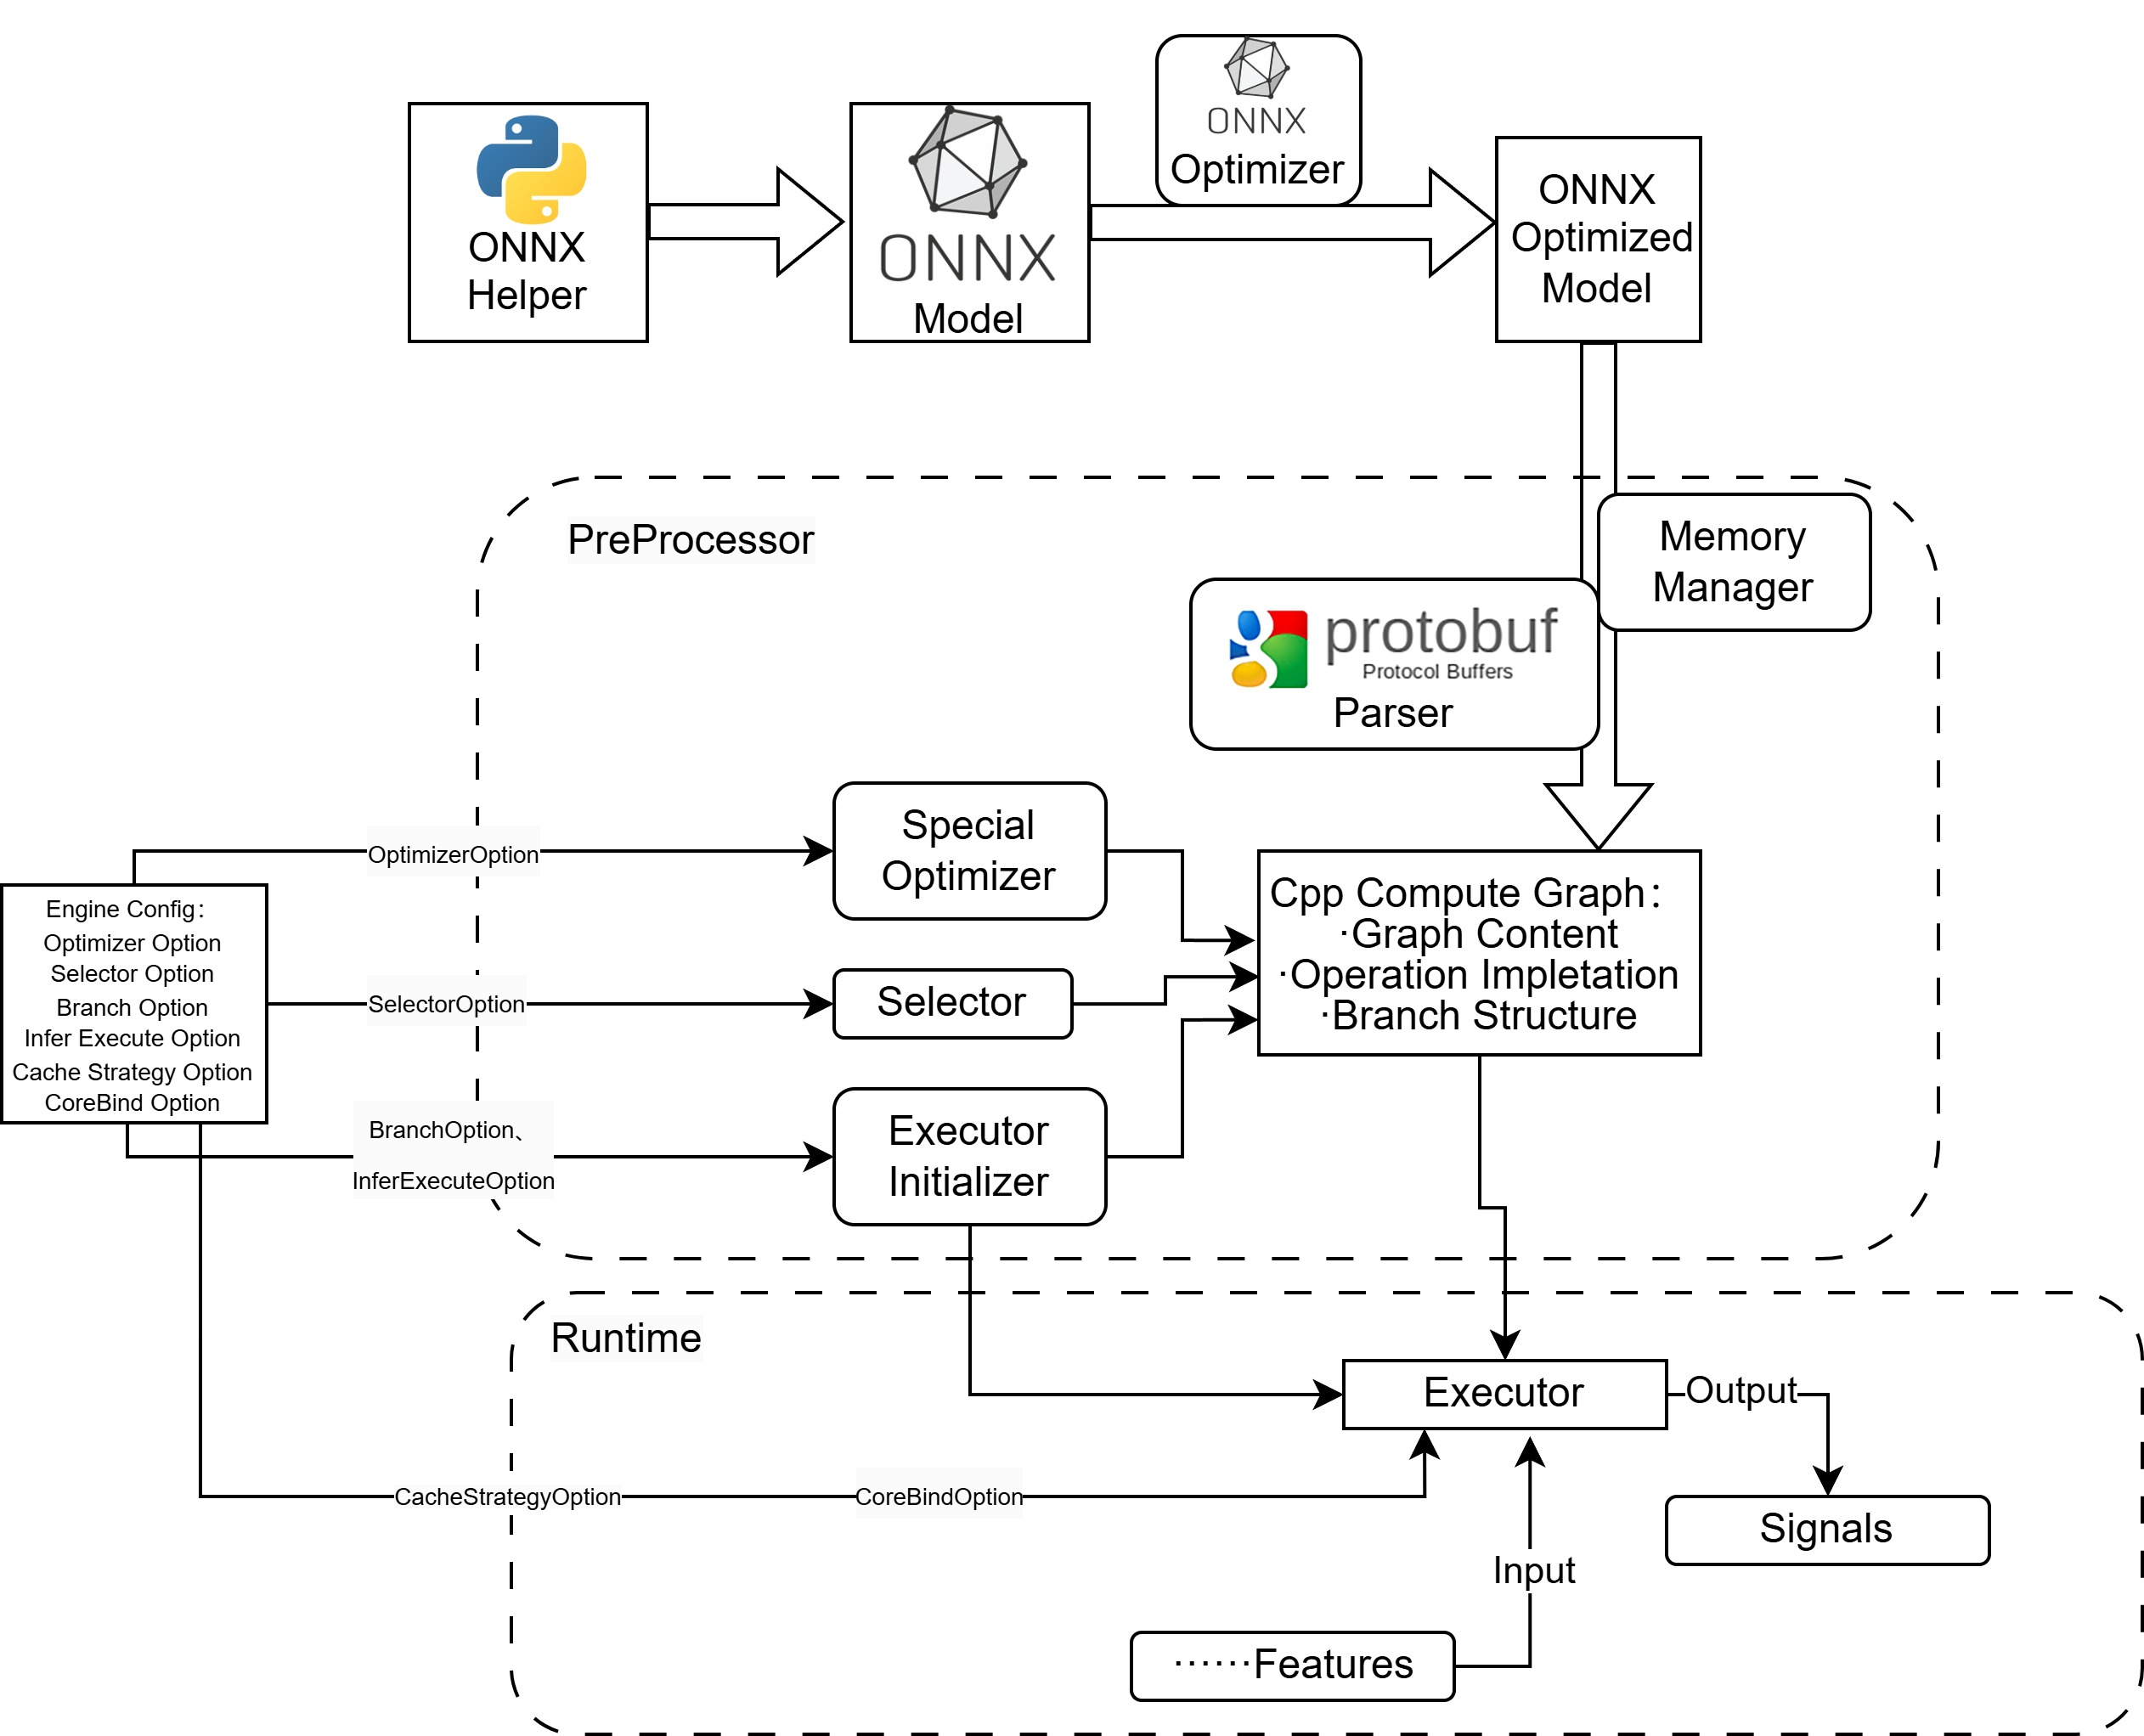
\includegraphics[width=0.9\textwidth]{image/chap03/framework.jpg}
    \caption{框架整体设计}
    \label{fig:hole}
\end{figure}

静态预处理阶段,其核心在于重建计算图并进一步实施多方面的优化。
在此阶段,通过采用Protobuf的高效序列化工具,能够将ONNX格式的机器学习模型解析并映射到C++类对象结构中。
这一过程不仅确保模型数据结构完整可用,也为后续优化操作提供对象基础和拓展空间。
在实际的优化流程中,研发人员依据既定的优化目标和需求,可以选择性地引入各类Pass。
例如,无效算子消除Pass能够识别并删除对模型最终输出结果无贡献的算子节点,从而有效简化计算图的结构;
算子融合Pass将多个在逻辑上紧密相连、在功能上可整合的算子进行合并,以此减少推理过程中的冗余访存和计算开销,提升计算资源的利用效率;
模型剪枝Pass通过去除模型中相对冗余的连接或节点,实现模型规模的削减,在不显著影响模型性能的前提下降低存储和计算负担;
量化Pass则专注于将模型中的高精度数据类型转换为低精度类型,从而在保证模型性能基本稳定的前提下,进一步提升计算效率,降低硬件资源的占用。
通过Optimizer中Pass的执行,推理框架能够像编译器一样对计算图独立开展优化,产生相对垂直的优化效果。
此外,静态预处理阶段还包含算子对硬件环境的适配与调优过程,能够基于目标设备的硬件配置细节,包括处理器架构、内存容量、缓存大小等关键参数,并依据这些信息对计算图中的各个算子进行针对性的调优和加速。
针对不同架构的处理器,可以优化算子的指令集使用,充分利用硬件的并行计算能力和缓存机制,以实现计算性能的最大化。
同时,本文提出的因子模型推理框架在静态预处理过程中,会基于配置请求预先完成分支分割和缓存算法等关键机制的基础设置。
其中,分支的拓扑分割操作依据模型的结构特点和运行需求,将复杂的计算图划分为多个相对独立且易于处理的子图分支,为后续的缓存应用和资源分配提供便利。

动态运行阶段则侧重对静态预处理之后所形成的各个组成部分进行高效的动态加载与运行。
在此过程中,核心隔离和绑定操作能够确保模型的不同部分在计算资源上实现合理分配与高效利用,避免资源冲突和浪费。
具体而言,通过将不同的计算任务绑定到特定的处理器核心或线程上并将核心隔离,可以使得极大减少由于系统进程调度导致的性能损失。
同时,分支缓存机制能够根据实际运行时的数据流情况,快速调整分支计算策略,保障模型运行保持高效。

综上所述,因子模型推理框架通过科学合理地结合静态预处理与动态运行这两个阶段,实现了局部优化与整体调度的协同提升。
这种将两者相分离的设计方案,在工程设计上降低了项目开发复杂度,为后续的优化工作开拓空间。
以此本文能够在此基础上,探索实现更多优化策略,推动因子模型推理性能提升,以适应日益复杂和多样化的应用场景需求。

\section{内存管理方法}

在高频交易场景下,多分支因子模型推理框架的运行依赖于高效的内存管理策略。
为了满足低延时的要求,推理框架采用了内存池(Memory Pool)和分配器(Allocator)相结合的内存管理机制。
这种机制通过预先分配大块内存并按需分配给计算图节点,显著减少了动态内存分配带来的延时开销,同时提高了内存使用的效率和稳定性。

内存池是推理框架内存管理的核心组件,其主要功能是预先分配一块大容量的内存空间,并在推理过程中按需分配给各个计算节点。
为了最大化内存访问速度并减少内存碎片化,内存池使用了mmap系统调用分配一个基于Huge Page的1GB内存区域。
Huge Page是一种操作系统提供的大页内存管理机制,通过减少页表项的数量,降低内存访问的TLB(Translation Lookaside Buffer)缺失率,从而显著提高内存访问速度。
在初始化阶段,推理框架通过mmap调用请求一个1GB的Huge Page内存区域,并将其映射到进程的地址空间。
这块内存被划分为多个固定大小的内存块,每个内存块对应一个计算图节点的内存需求。
内存池维护一个指针,指向当前可分配内存的起点。每次分配内存时,内存池通过更新该指针的位置来分配连续的内存块,从而避免了传统动态内存分配算法中的锁竞争和内存碎片化问题。
内存池的设计还有助于提高系统的可扩展性,便于根据不同的硬件配置和应用场景进行灵活调整,确保在不同环境下都能实现最优的内存管理效果。

内存分配器是内存池的管理接口,负责将内存池中的内存分配给具体的计算图节点。
在推理框架的预处理阶段,计算图的每个节点会根据其输入和输出张量(Tensor)的大小向分配器请求内存。
分配器根据节点的请求,从内存池中分配相应的内存块,并将内存的起始地址返回给节点。
在张量初始化时,推理框架会根据张量的形状和数据类型计算所需的内存大小,并通过分配器从内存池中申请内存。
分配器会检查内存池中是否有足够的连续内存块可供分配。
如果有,则更新内存池的起点指针,将内存块分配给张量;如果没有,则返回错误。
分配器还具备智能分配策略,能够根据节点的优先级和内存需求的紧急程度,合理分配内存资源,确保关键节点的内存供应,从而进一步提升系统的整体性能和可靠性。
此外,分配器在内存回收方面也进行了优化,对于不再使用的内存块能够及时释放并归还给内存池,以供其他节点重新使用,进一步提高了内存的利用率。

为了进一步优化内存管理的性能,推理框架在初始化结束后固定已分配的内存区域。
这一策略基于高频交易场景下模型输入和输出张量大小相对固定的特点。
在初始化阶段,推理框架会一次性分配足够的内存。一旦初始化完成,内存池中的内存分配便不再变化,从而避免了运行时的动态内存分配和回收操作。
此外,推理框架还通过内存锁定机制(Memory Locking)将分配的内存锁定在物理内存中,防止操作系统将这些内存页交换到磁盘。
这不仅减少了内存访问的延迟,还提高了系统的稳定性,确保在高频交易的高负载场景下不会因内存交换而引入额外的延时。
这种固定的内存分配策略还有助于提高系统的可预测性,便于对内存使用情况进行监控和优化,为系统的长期稳定运行提供有力保障。
同时,通过固定内存区域,可以有效减少因内存分配和回收频繁操作而导致的系统开销,使得推理框架能够更加专注于模型的计算和推理任务,从而在高频交易中快速响应市场变化,做出精准的交易决策。

\begin{figure}[h]
    \centering
    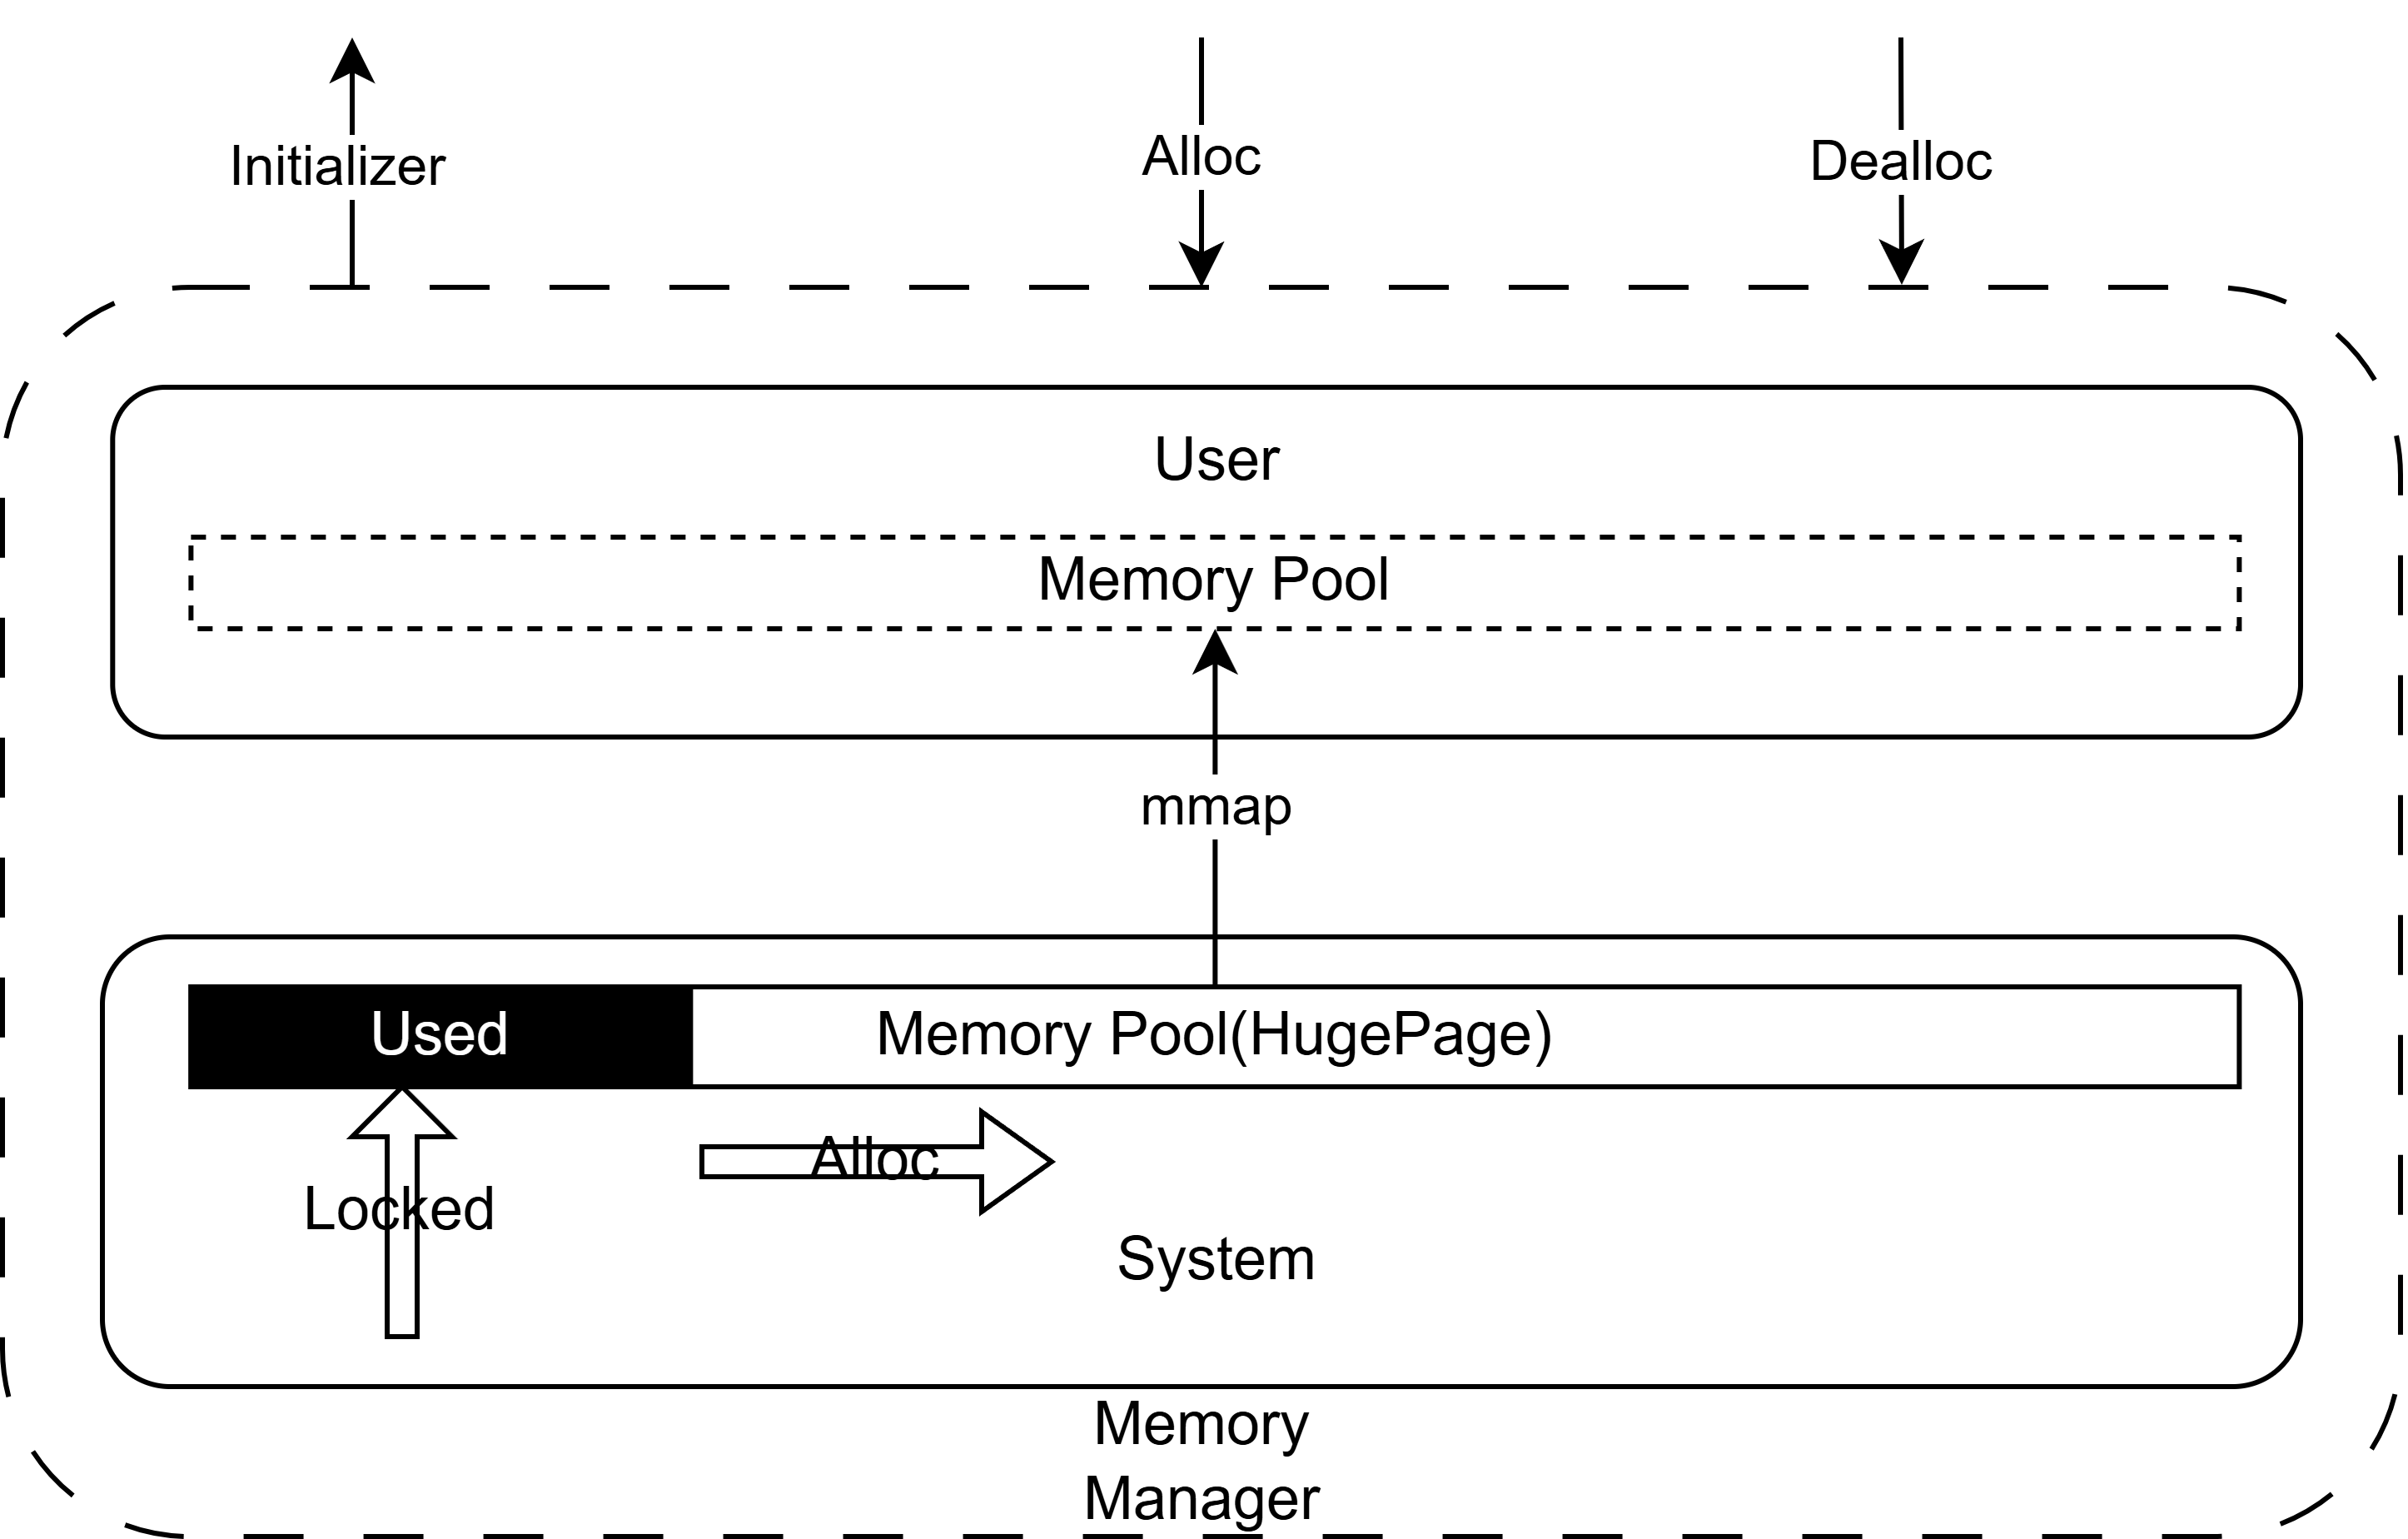
\includegraphics[width=0.9\textwidth]{image/chap03/memmory.png}
    \caption{内存管理器}
    \label{fig:hole}
\end{figure}

推理框架的内存管理机制通过内存池和分配器的设计,结合Huge Page和内存锁定技术,有效解决了高频交易场景下低延时和高效率的内存管理需求。
这种机制不仅减少了动态内存分配的开销,还提高了内存访问的速度和稳定性,为高频交易中的多分支因子模型推理提供了强大的支持。
在实际应用中,该内存管理机制能够显著提升推理框架的性能表现,使其在高频交易领域中具备显著的竞争优势,能够更有效地处理大规模数据和模型推理任务。

\section{算子调优与绑定}
在高频交易业务场景下,程序自动交易链路的全过程对延时的要求极为苛刻,关键路径的最大延时必须被约束在数十乃至数微秒。
这一延时标准直接决定了量化策略是否能够在指定价格位置准确执行交易,否则可能导致显著的损失。
因此,作为关键路径中延时的主要来源,因子模型的计算过程必须充分利用硬件性能以减小延时,其中算子的调优是至关重要的环节。

在此前提下,框架提供了算子调优与绑定的简易步骤,加速了框架应用于目标硬件的部署实践。
首先,框架在Blaze HPC编译过程中结合Intel MKL、AMD AOCL等数学库与CPU架构信息,如各级缓存大小、指令集等,从而在算子性能本身提供最优实践。
其次,对于Blaze HPC不支持的进一步优化,在部署框架过程中,框架通过Selector类可以综合计算需求和CPU信息来动态绑定算子。
例如,Intel GEMM JIT对于小规模浮点数矩阵乘有显著加速效果,框架通过判定指定节点的计算类型和规模,可将该节点算子绑定到Intel GEMM JIT。
因此,算子绑定过程具有极大的可拓展性,对于先进的计算优化也可以通过简单的拓展开发进行快速适配。
同样,模型经过静态优化器可以产生节点的融合,对于此类非常规的算子,BLAS通常不能提供支持,但框架仍然支持通过简易的拓展开发实现手写算子,只需要使用CPU定制编译器如ICPX等进行目标架构的针对性优化即可。
通过上述算子的调优与绑定过程,算子执行得以充分利用硬件的性能,极大提高了因子模型的推理效率。

具体到指令集覆盖方面,在CPU算子优化过程中,充分利用现代CPU的指令集和架构特性是提高性能的关键。
特别是AVX2和AVX-512指令集,它们能够显著提升数据的并行处理能力。
AVX2支持256位的向量化操作,而AVX-512则进一步扩展到512位,理论上能够提供更高的计算效率。
然而,在实际应用中,AVX-512的性能提升并不总是显著的,尤其是在某些特定型号的CPU上。
例如,对于AMD EPYC系列CPU,虽然其支持AVX-512指令集,但在某些场景下,使用AVX-512可能会导致CPU积热,从而触发降频机制,反而降低了整体性能。
为了避免这种情况,优化策略中需要根据具体的CPU型号和应用场景灵活选择指令集。
例如,在AMD EPYC平台上,可以优先选择AVX2指令集,以避免因积热导致的降频问题。这种策略不仅能够保证CPU在高频交易场景下的稳定运行,还能充分利用硬件的计算能力。

在实际的交易场景中,这种优化策略的实施包含多个过程。
首先,需要对不同的CPU型号进行详细的性能测试,以确定在特定工作负载下哪种指令集能够提供最佳的性能表现。
这既包括对不同指令集在矩阵运算、浮点运算等常见计算任务中的执行时间、能耗以及温度变化的监测,
又要考虑交易系统的整体架构,包括数据传输、任务调度以及与其他系统组件的交互,确保算子优化不会引入新的瓶颈。
通过针对硬件性能的细粒度优化,可以确保高频交易系统在市场竞争中保持性能优势,实现高效的交易执行和风险控制。
\section{分支拓扑分割算法}
\begin{figure}[h]
    \centering
    \includegraphics[width=0.9\textwidth]{image/chap03/branchs.jpg}
    \caption{分支拓扑分割算法中以分支为单位的计算图重建}
    \label{fig:hole}
\end{figure}
在量化交易中,多分支因子模型被广泛应用以生成交易信号。
这些模型的输入通常由多个市场特征拼接而成,这些特征在前序步骤中经计算操作,进入模型后被切分到不同分支中处理。
尽针对管不同交易品类所设计的多分支因子模型在具体设计上存在较大差异,
但整体上,各个分支在经过一定处理后,都会通过通用矩阵乘法(GEMM)映射到高维空间,然后各分支之间通过计算操作逐级合并,最终得到一个输出。
从形状上看,这种模型结构类似于一个从叶子到根的树状收敛结构。
\begin{wrapfigure}{r}{0.4\linewidth}
    \centering
    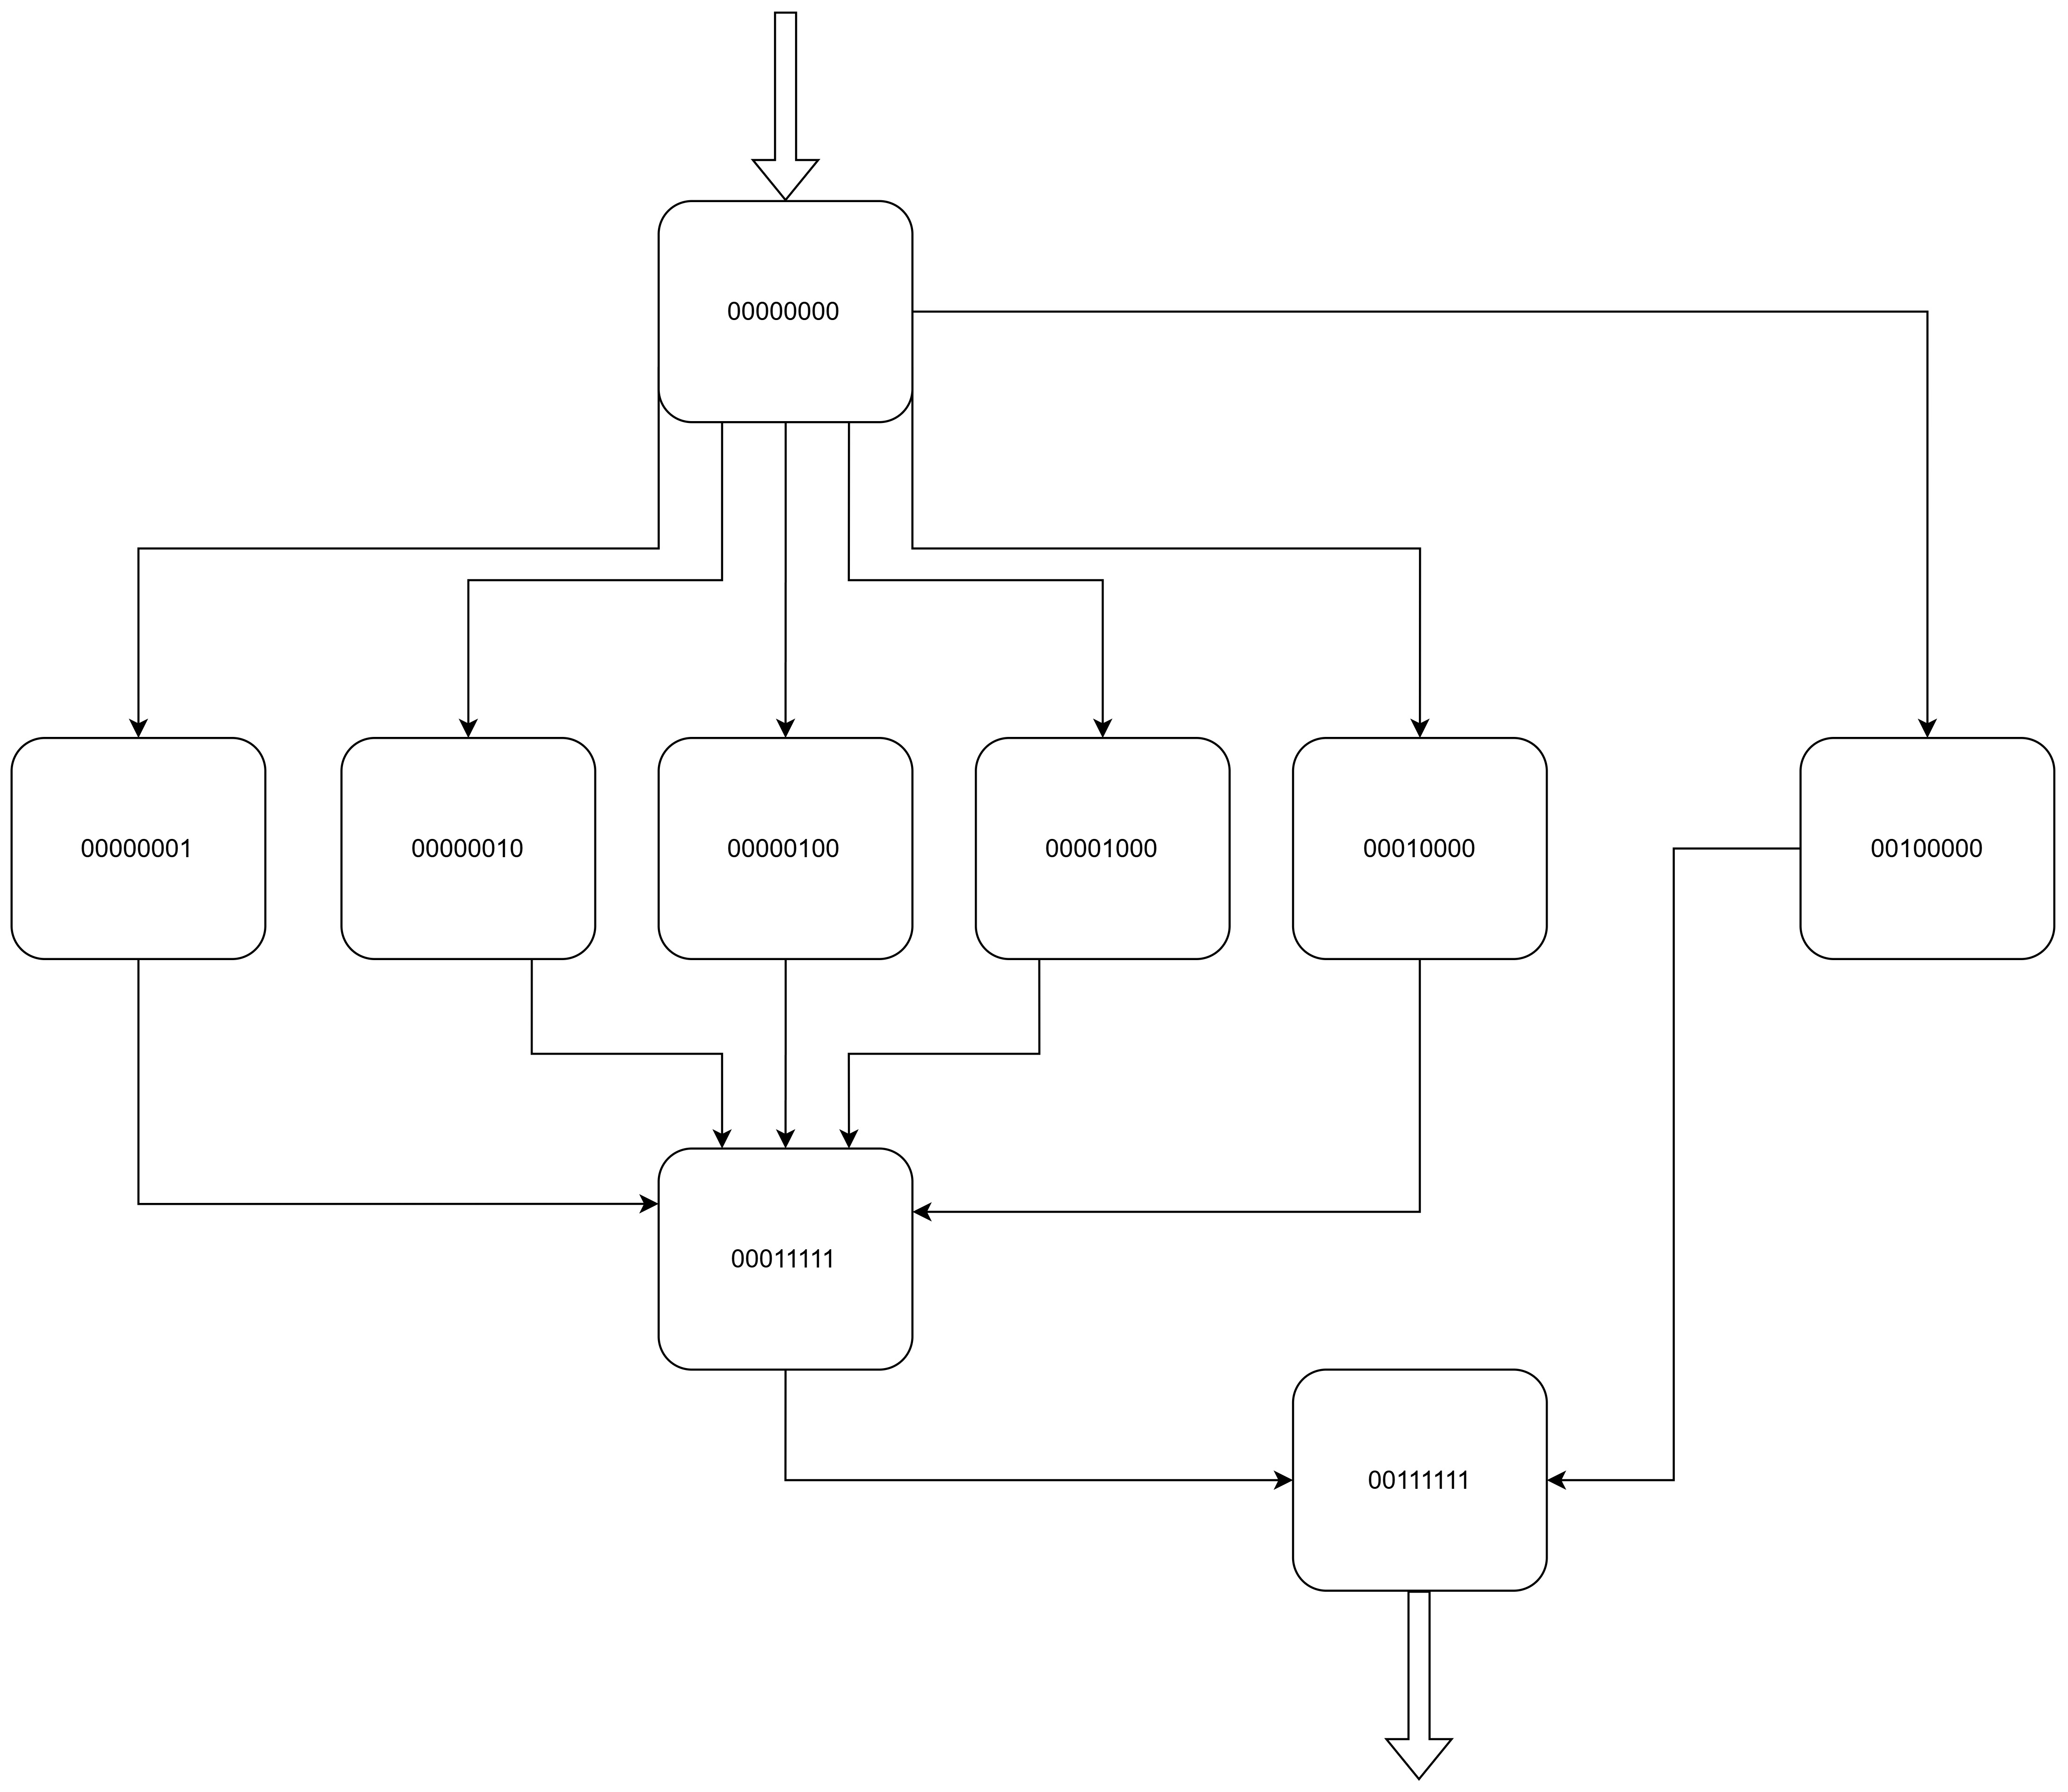
\includegraphics[width=0.4\textwidth]{image/chap03/branch2.jpg}
    \caption{分支位标记示意图}
    \label{fig:image-embedding-text}
\end{wrapfigure}
为了优化模型的推理过程,我们利用位运算来标记各个分支,
并通过这种方式,将以节点为单位的计算图重建为以分支为单位的计算图。
这种重建不仅有助于清晰地展示模型的逻辑结构,还为后续的分支缓存算法提供了必要的支持,从而加速模型的计算。
同时,在工程设计方面,分支的拓扑分割为模型优化提供了图和节点除外的新粒度,使得计算图在分支这一抽象层具有更多优化空间。


算法流程如下所示:
\begin{algorithm}[h]
    \KwIn{计算图G,输入节点集合InputNodes,分支初始节点集合BranchStartNodes}
    \KwOut{以分支为单位的计算图结构PartitionedGraph}
    \textbf{初始化:}\;
    \For{输入节点$InputNode$ in $InputNodes$}{
        \For{切片操作$SliceOpNode$ in $InputNode$.$ChildNodes$}{
            为每个分支初始节点分配一个唯一的位标记$BitMask$,如$BitMask = 1 << index$\;
        }
    }
    
    \textbf{深度优先搜索标记传播:}\;
    \For{分支初始节点$BranchNode$ in $BranchStartNodes$}{
        初始化当前分支标记$CurrentBitMask = BranchNode$.位标记\;
        \textbf{深度优先搜索:}\;
        \For{子节点$ChildNode$ in $BranchNode$.$ChildNodes$集合}{
            $ChildNode$.$BitMask |= CurrentBitMask$\;
            递归地对$ChildNode$的子节点进行相同操作\;
        }
    }
    \textbf{深度优先搜索计算图重建:}\;
    初始化当前位标记$CurrentBitMask = 0$\;
    当前节点为$CurrentNode = InputNodes$\;
    当前分支为$InputNodes$组成的初始分支$CurrentBranch = InputBranch$,然后深度优先搜索子节点;
    \For{$Node$ in $CurrentNode$.$ChildNodes$}{
    \If{$Node$.$BitMask$ != $CurrentNode$.$BitMask$}{
        创建新的分支$NewBranch$;
        $CurrentBranch$.$ChildBranch$加入$NewBranch$;
        $CurrentBranch$ = $NewBranch$;
        $CurrentNode$.$BitMask$ = $Node$.$BitMask$
    }
    将$Node$添加到$NewBranch$;
    递归地对$Node$.$ChildNodes$进行相同操作;
    }
    将所有分支整合到PartitionedGraph中;

    \caption{分支拓扑分割算法}
    \label{algo:branch_topology_partitioning}
\end{algorithm}

这样,在模型推理过程中,可以针对每个分支进行独立的优化操作,例如缓存管理、资源分配等,从而拓展优化空间。
利用位运算标记分支,我们可以将以节点为单位的计算图重建为以分支为单位的计算图,用以支持之后的分支缓存算法加速计算。

\section{分支缓存机制}

\subsection{基于实时行情的分支缓存}

在实际的高频交易场景中,在最高级别的实时行情(Full Tick)下,该交易品类下所有交易操作都会实时发送到低延时系统更新和处理。
此类行情更新虽然具有优越的实时性和最详尽的行情数据,但是另一方面任意交易者的所有操作都会触发交易系统的一轮执行,带来了极高的计算压力。
然而,并不是所有交易操作都会对因子模型的特征输入产生影响,例如偏离最优成交价格的预埋单,并不会影响因子模型对于行情的基本特征提取。
这意味着尽管交易因子模型仍然必须在行情更新时进行推理,但是其部分特征输入在多数情况下不受行情数据中噪声操作更新影响。
而此类对行情变化不敏感的特征输入对应部分分支的计算过程就存在优化空间。

框架使用分支拓扑分割方法基于分支重建了模型计算图。
通过在分支推理函数中添加分支输入与缓存的上一次输入匹配函数,可以在缓存命中的条件下可以将上次计算结果返回输出。
此类方法不仅对于输入特征本身的数据格式没有特殊要求,
而且在高频场景下每秒的数万次行情操作更新中,多数操作实际为行情噪声,仅有少数趋势成交导致行情特征数值变化从而影响因子模型推理。
\begin{figure}[h]
    \centering
    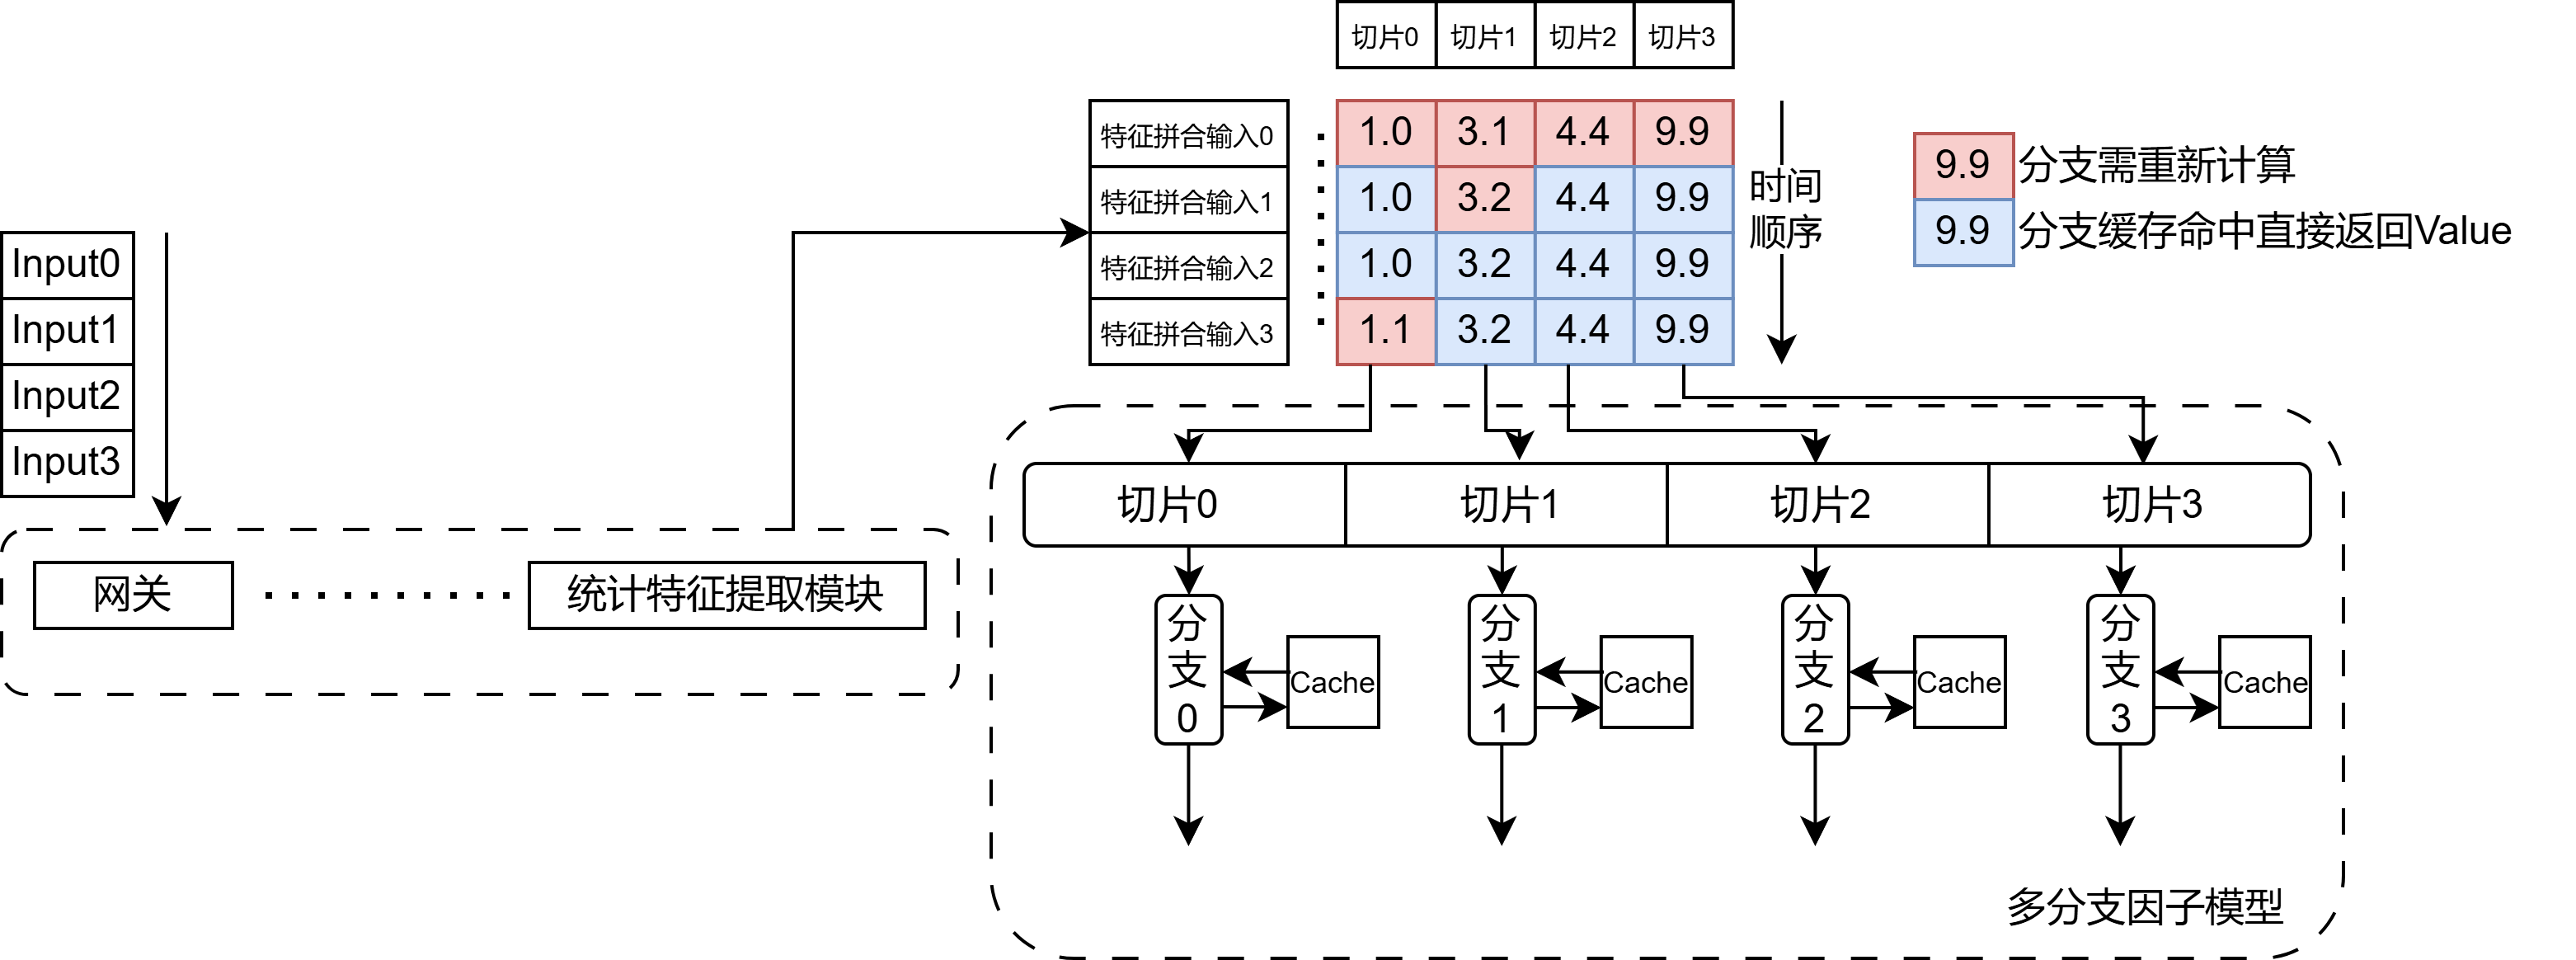
\includegraphics[width=1\textwidth]{image/chap03/high.png}
    \caption{实时行情中缓存加速}
    \label{fig:hole}
\end{figure}


\subsection{基于可枚举输入特征的预计算分支缓存}

以当前成交价格为例,在期货交易市场中,每个交易品类都有一个最小价格波动单位。
除极少的黑天鹅事件外,单个交易日内的价格波动通常在一定范围内。
例如,对于沪铝2503合约,其最小价格波动为5元/吨,而实际交易中单个交易日内价格波动极少超过500元。
基于这一特性,框架通过在盘前预计算并缓存100个波动输入值,为交易日当天所有的成交价格情况做预计算。
这样,在整个交易日内,模型可以直接从缓存中获取这些预计算的值,从而显著减少计算时间。
具体而言,对沪铝2503成交价格的特征输入进行缓存的方法的内存占用较小,通常不多于10KB。
为了实现这一优化,在上述分支拓扑分割算法执行后,框架为每一个分支加入缓存机制。
当市场数据输入与缓存中的数据匹配时,模型直接从缓存中检索预计算的输出,并将其传递给后续节点。
类似的,对于低精度如FP16等数据格式的因子输入,由于多数行情特征为单一值,
因此存在枚举FP16所有取值并预计算分支输出从而建立缓存,将分支推理直接简化为哈希表查询过程的缓存方案。
这不仅减少了冗余计算,还加速了整体的推理过程。
\begin{figure}[h]
    \centering
    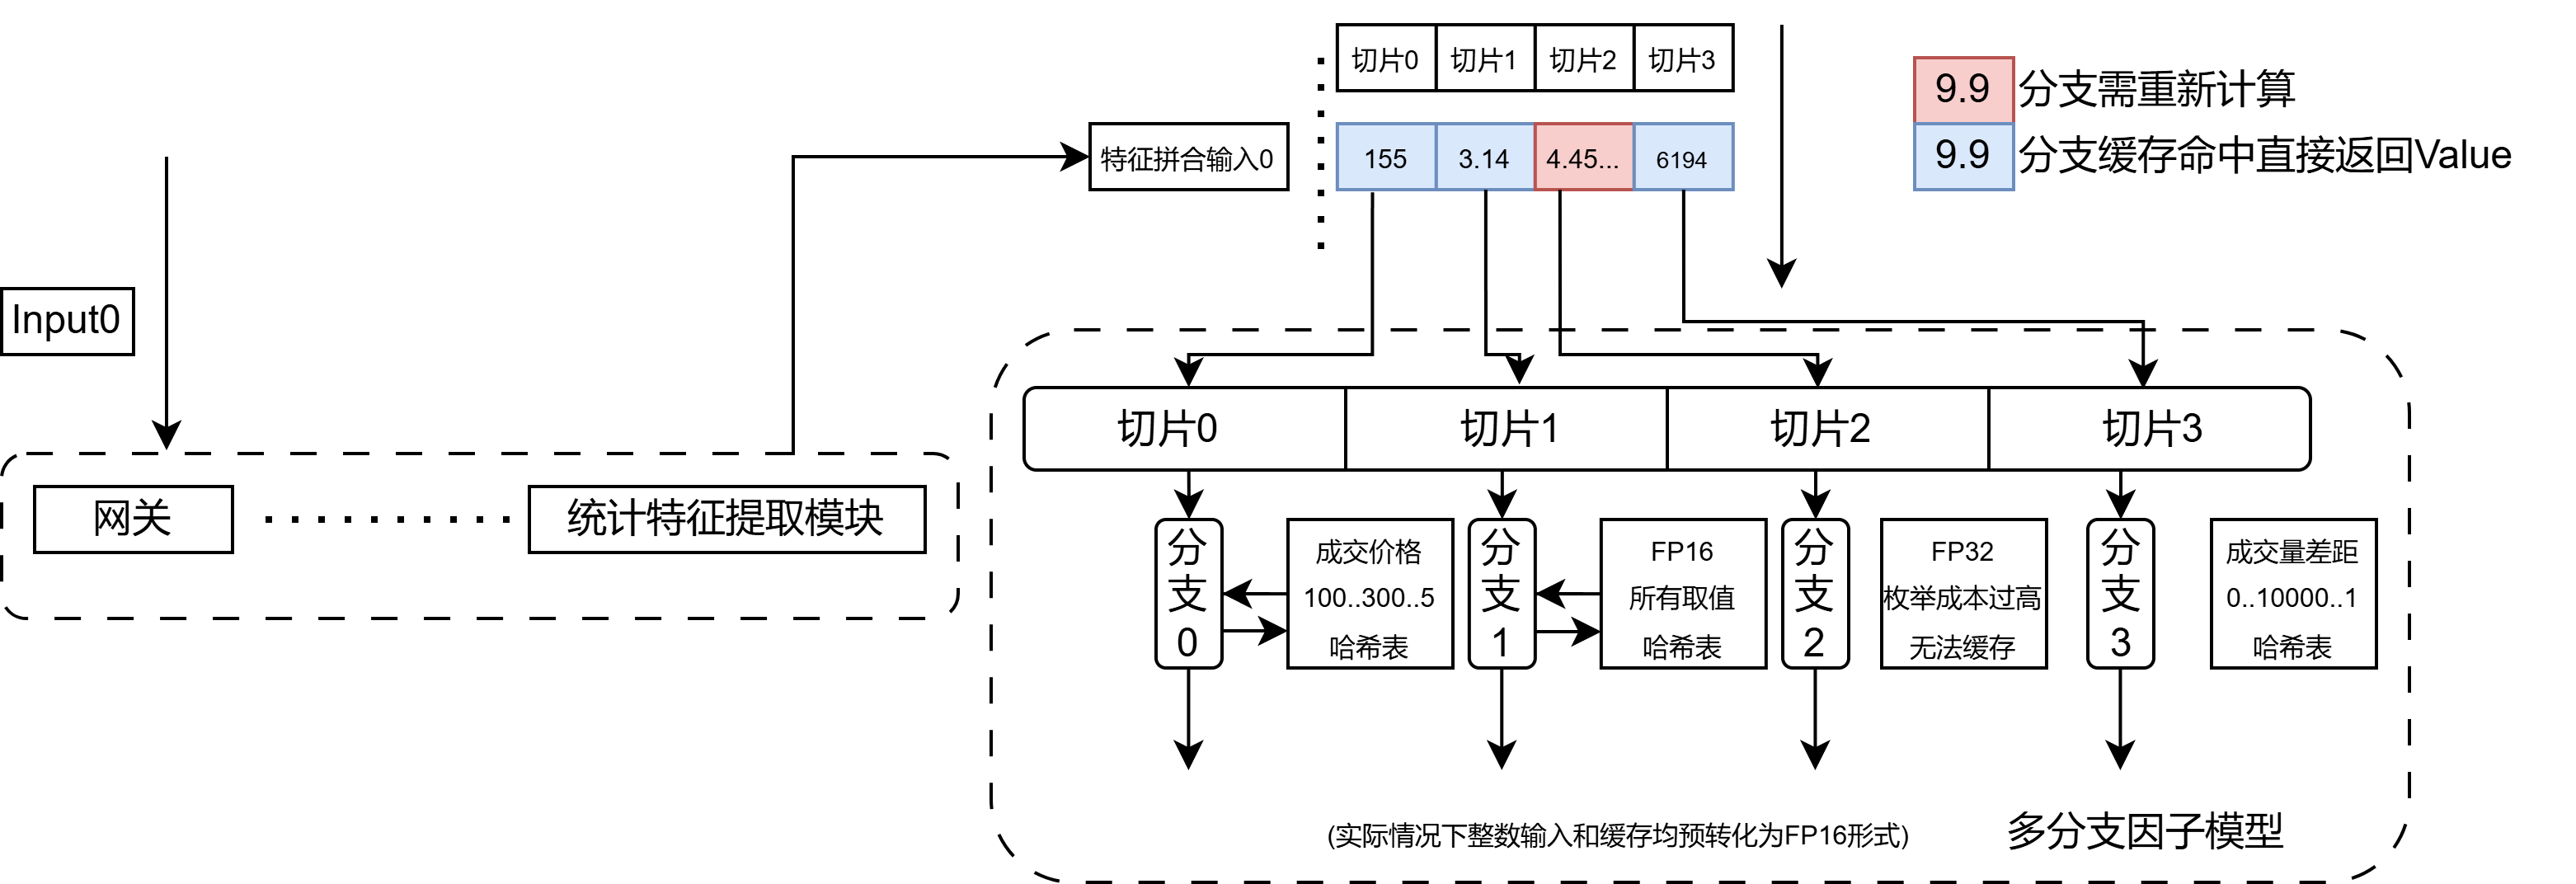
\includegraphics[width=1\textwidth]{image/chap03/precom.png}
    \caption{预计算分支缓存}
    \label{fig:hole}
\end{figure}

\subsection{缓存机制的选取}

实现缓存机制尽管在多数情况下能够实现分支计算过程的简化加速,
但是对于高频交易系统,缓存机制作为分支抽象层的附加实现,需要考虑在缓存未命中条件下的执行延时增加。
而在CPU缓存和系统内存缓存中常用的LRU与FIFO等机制,其需要维护动态缓存池,
相比较匹配上一次输入和预计算固定缓存查询具有较高的延时成本,即便通过维护动态缓存池可能有效提高缓存命中率,但是无缓存命中情况下的推理延时显著增加。
因此缓存机制只使用匹配上一次输入和预计算固定缓存查询两种高效缓存方法,其相比较原推理过程不仅通过缓存命中大幅减少推理延时,在无缓存命中情况下的推理延时几乎没有增加。

综上所述,选择合适的缓存替换机制需要综合考虑市场数据的特性、系统的内存资源以及模型的计算复杂度。
在实际应用中,可以根据具体的交易场景和系统配置,灵活地选择或组合这些缓存策略,以达到最优的性能表现。
在不同的市场条件下,市场数据的特征可能会发生变化,因此需要定期对缓存策略进行评估和调整,以确保其始终能够适应当前的市场环境。
同时,考虑到交易系统的实时性和稳定性要求,缓存机制的实现还需要充分考虑数据的一致性和准确性,避免因缓存数据的错误或过时而导致交易决策的失误。
此外,随着交易规模的扩大和市场数据量的增加,缓存机制的扩展性和可维护性也变得尤为重要,需要在系统设计阶段就充分考虑这些因素,以保证交易系统的长期稳定运行和高效性能。